% !TeX spellcheck = en_US
% !TeX encoding = UTF-8
\documentclass[10pt, a4paper, landscape]{article}

% ----- packages -----
\usepackage{amsmath} % AMS mathematical facilities for LaTeX
\usepackage{enumitem} % Control layout of itemize, enumerate, description
\usepackage{fancyhdr} % Extensive control of page headers and footers in LaTeX2
\usepackage{geometry} % Flexible and complete interface to document dimensions
\usepackage{graphicx} % Enhanced support for graphics
\usepackage{hyperref} % Extensive support for hypertext in LaTeX
\usepackage{multicol} % Intermix single and multiple columns
\usepackage{parskip} % Layout with zero \parindent, non-zero \parskip
\usepackage{tikz} % Create PostScript and PDF graphics in TeX
\usepackage{titlesec} % Select alternative section titles

% ----- pdf metadata -----
\hypersetup{
	pdftitle={Time Series Cheat Sheet},
	pdfsubject={The Econometrics Cheat Sheet Project - marcelomijas - CC-BY-4.0},
	pdfauthor={Marcelo Moreno Porras},
	pdfkeywords={statistics, latex, economics, cheatsheet, econometrcis, ols-regression, economic-modelling},
	pdfduplex={DuplexFlipShortEdge}
}

% ----- random seed -----
\pgfmathsetseed{12}

% ----- custom commands -----
\DeclareMathOperator{\E}{E}
\DeclareMathOperator{\Var}{Var}
\DeclareMathOperator{\se}{se}
\DeclareMathOperator{\Cov}{Cov}
\DeclareMathOperator{\Corr}{Corr}

% ----- page customization -----
\geometry{margin=1cm} % margins config
\pagenumbering{gobble} % remove page numeration
\setlength{\parskip}{0cm} % paragraph spacing
% title spacing
\titlespacing{\section}{0pt}{2ex}{1ex}
\titlespacing{\subsection}{0pt}{1ex}{0ex}
\titlespacing{\subsubsection}{0pt}{0.5ex}{0ex}

% ----- footer -----
\pagestyle{fancy}
\renewcommand{\headrulewidth}{0pt}
\cfoot{\href{https://github.com/marcelomijas/econometrics-cheatsheet}{\normalfont \footnotesize TS-25.08.1-EN - github.com/marcelomijas/econometrics-cheatsheet - CC-BY-4.0 license}}
\setlength{\footskip}{12pt}

% ----- document -----
\begin{document}

\begin{multicols}{3}

\begin{center}
	\textbf{\LARGE \href{https://github.com/marcelomijas/econometrics-cheatsheet}{Time Series Cheat Sheet}}

	{\footnotesize By Marcelo Moreno Porras - Universidad Rey Juan Carlos}

	{\footnotesize The Econometrics Cheat Sheet Project}
\end{center}

\section*{Basic concepts}

\subsection*{Definitions}

\textbf{Time series} - succession of observations ordered in time with a fixed frequency.

Given the format of a time series:

\begin{itemize}[leftmargin=*]
	\item \textbf{Point-in-time (stock)} - a single value is recorded for each period.
	\item \textbf{Aggregated (flow)} - values represent totals or averages over the period.
	\item \textbf{Range/interval (OHLC)} - each period records multiple summary statistics, such as min, max, open, close.
\end{itemize}

\textbf{Stochastic process} - a sequence of random variables that are indexed in time.

\subsection*{Components of a time series}

\begin{itemize}[leftmargin=*]
	\item \textbf{Trend} - the long-term general movement of a series.
	\item \textbf{Seasonal variations} - periodic oscillations that are produced in a period equal to or inferior than a year, and can be easily identified across different years (usually the result of climatology).
	\item \textbf{Cyclical variations} - periodic oscillations that are produced in a period greater than a year (are the result of the economic cycle).
	\item \textbf{Residual variations} - movements that do not follow a recognizable periodic oscillation (irregular events).
\end{itemize}

\subsection*{Type of time series models}

\begin{itemize}[leftmargin=*]
	\item \textbf{Static models} - the relation between \( y \) and \( x \) is contemporary. Conceptually:
	\begin{center}
		\( y_{t} = \beta_{0} + \beta_{1} x_{t} + u_{t} \)
	\end{center}
	\item \textbf{Distributed-lag models} - the relation between \( y \) and \( x \) is not contemporary. Conceptually:
	\begin{center}
		\( y_{t} = \beta_{0} + \beta_{1} x_{t} + \beta_{2} x_{t - 1} + \cdots + \beta_{s} x_{t - (s - 1)} + u_{t} \)
	\end{center}
	The long-term cumulative effect in \( y \) when \( \Delta x \) is:
	\begin{center}
		\( \beta_{1} + \beta_{2} + \cdots + \beta_{s} \)
	\end{center}
	\item \textbf{Dynamic models} - lags of the dependent variable (endogeneity). Conceptually:
	\begin{center}
		\( y_{t} = \beta_{0} + \beta_{1} y_{t - 1} + \cdots + \beta_{s} y_{t - s} + u_{t} \)
	\end{center}
		\item Combinations of the above, like the rational distributed-lag models (distributed-lag + dynamic).
\end{itemize}

\columnbreak

\section*{Assumptions and properties}

\subsection*{OLS model assumptions under time series}

Under these assumptions, the OLS estimator will present good properties. \textbf{Gauss-Markov assumptions} extended for time series:

\begin{enumerate}[leftmargin=*, label=t\arabic{*}.]
	\item \textbf{Parameters linearity and weak dependence}.
	\begin{enumerate}[leftmargin=*, label=\alph{*}.]
		\item \( y_{t} \) must be a linear function of the \( \beta \)'s.
		\item The stochastic \( \lbrace (x_{t}, y_{t}) : t = 1, 2, \ldots, T \rbrace \) is stationary and weakly dependent.
	\end{enumerate}
	\item \textbf{No perfect collinearity}.
	\begin{itemize}[leftmargin=*]
		\item There are no independent variables that are constant: \( \Var(x_{j}) \neq 0, \; \forall j = 1, \ldots, k \)
		\item There is no exact linear relation between independent variables.
	\end{itemize}
	\item \textbf{Conditional mean zero and correlation zero}.
	\begin{enumerate}[leftmargin=*, label=\alph{*}.]
		\item There are no systematic errors: \( \E(u \mid x_{1}, \ldots, x_{k}) = \E(u) = 0 \rightarrow \) \textbf{strong exogeneity} (a implies b).
		\item There are no relevant variables left out of the model: \( \Cov(x_{j} , u) = 0, \; \forall j = 1, \ldots, k \rightarrow \) \textbf{weak exogeneity}.
	\end{enumerate}
	\item \textbf{Homoscedasticity}. The variability of the residuals is the same for any \( x \): \( \Var(u \mid x_{1}, \ldots, x_{k}) = \sigma_{u}^{2} \)
	\item \textbf{No autocorrelation}. Residuals do not contain information about any other residuals: \\
	\( \Corr(u_{t}, u_{s} \mid x_{1}, \ldots, x_{k}) = 0, \; \forall t \neq s \)
	\item \textbf{Normality}. Residuals are independent and identically distributed (\textbf{i.i.d.}): \( u \sim \mathcal{N} (0, \sigma_{u}^{2}) \)
	\item \textbf{Data size}. The number of observations available must be greater than \( (k + 1) \) parameters to estimate. (It is already satisfied under asymptotic situations)
\end{enumerate}

\subsection*{Asymptotic properties of OLS}

Under the econometric model assumptions and the Central Limit Theorem:

\begin{itemize}[leftmargin=*]
	\item Hold t1 to t3a: OLS is \textbf{unbiased}. \( \E(\hat{\beta}_{j}) = \beta_{j} \)
	\item Hold t1 to t3: OLS is \textbf{consistent}. \( \operatorname{plim}(\hat{\beta}_{j}) = \beta_{j} \) (to t3b left out t3a, weak exogeneity, biased but consistent)
	\item Hold t1 to t5: \textbf{Asymptotic normality} of OLS (then, t6 is necessarily satisfied): \( u \underset{a}{\sim} \mathcal{N} (0, \sigma_{u}^{2}) \)
	\item Hold t1 to t5: \textbf{Unbiased estimate} of \( \sigma_{u}^{2} \). \( \E(\hat{\sigma}_{u}^{2}) = \sigma^{2}_{u} \)
	\item Hold t1 to t5: OLS is \textcolor{blue}{BLUE} (Best Linear Unbiased Estimator) or \textbf{efficient}.
	\item Hold t1 to t6: Hypothesis testing and confidence intervals can be done reliably.
\end{itemize}

\columnbreak

\section*{Trends and seasonality}

\textbf{Spurious regression} - is when the relation between \( y \) and \( x \) is due to factors that affect \( y \) and have a correlation with \( x \), \( \Corr(x_{j}, u) \neq 0 \). Is the \textbf{non-fulfillment of t3}.

\subsection*{Trends}

Two time series can have the same (or contrary) trend, which should lead to a high level of correlation. This can provoke a false appearance of causality; the problem is \textbf{spurious regression}. Given the model:

\begin{center}
	\( y_{t} = \beta_{0} + \beta_{1} x_{t} + u_{t} \)
\end{center}

where:

\begin{center}
	\( y_{t} = \alpha_{0} + \alpha_{1} \text{Trend} + v_{t} \)

	\( x_{t} = \gamma_{0} + \gamma_{1} \text{Trend} + v_{t} \)
\end{center}

Adding a trend to the model can solve the problem:

\begin{center}
	\( y_{t} = \beta_{0} + \beta_{1} x_{t} + \beta_{2} \text{Trend} + u_{t} \)
\end{center}

The trend can be linear or non-linear (quadratic, cubic, exponential, etc.)

Another way is to make use of the \textbf{Hodrick-Prescott filter} to extract the trend and the cyclical component.

\subsection*{Seasonality}

\setlength{\multicolsep}{0pt}
\begin{multicols}{2}

A time series with can manifest seasonality. That is, the series is subject to a seasonal variations or patterns, usually related to climatology conditions.

\columnbreak

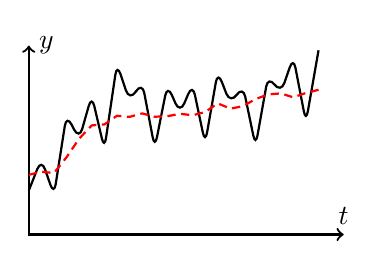
\begin{tikzpicture}[scale=0.20]
	\draw [thick, <->] (0, 12) node [anchor=west] {\( y \)} -- (0, 0) -- (20, 0) node [anchor=south] {\( t \)};
	\draw [thick, black, rounded corners] 
	(0.0, 2.79) -- (0.8, 4.81) -- 
	(1.6, 2.50) -- (2.4, 7.61) -- 
	(3.2, 6.03) -- (4.0, 8.84) -- 
	(4.8, 5.42) -- (5.6, 10.85) -- 
	(6.4, 8.47) -- (7.2, 9.69) -- 
	(8.0, 5.48) -- (8.8, 9.51) -- 
	(9.6, 7.68) -- (10.4, 9.57) -- 
	(11.2, 5.78) -- (12.0, 10.36) -- 
	(12.8, 8.29) -- (13.6, 9.45) -- 
	(14.4, 5.60) -- (15.2, 10.09) -- 
	(16.0, 8.96) -- (16.8, 11.28) -- 
	(17.6, 7.13) -- (18.4, 11.70);
	\draw [thick, red, densely dashed, line join=round] 
	(0.0, 3.79) -- (0.8, 3.99) -- 
	(1.6, 3.90) -- (2.4, 4.91) -- 
	(3.2, 6.09) -- (4.0, 6.93) -- 
	(4.8, 6.99) -- (5.6, 7.54) -- 
	(6.4, 7.47) -- (7.2, 7.69) -- 
	(8.0, 7.48) -- (8.8, 7.51) -- 
	(9.6, 7.67) -- (10.4, 7.57) -- 
	(11.2, 7.78) -- (12.0, 8.33) -- 
	(12.8, 7.99) -- (13.6, 8.15) -- 
	(14.4, 8.60) -- (15.2, 8.90) -- 
	(16.0, 8.96) -- (16.8, 8.71) -- 
	(17.6, 8.99) -- (18.4, 9.19);
\end{tikzpicture}

\end{multicols}

For example, GDP (black) is usually higher in summer and lower in winter. Seasonally adjusted series ({\color{red} dashed red}) for comparison.

\begin{itemize}[leftmargin=*]
	\item Regressing time series that present seasonality can lead to \textbf{spurious results}.
\end{itemize}

A simple \textbf{seasonal adjustment} could be creating stationary binary variables and adding them to the model. For example, for quarterly series (\( Q q_{t} \) are binary variables):

\begin{center}
	\( y_{t} = \beta_{0} + \beta_{1} Q2_{t} + \beta_{2} Q3_{t} + \beta_{3} Q4_{t} + \beta_{4} x_{1t} + \cdots + \beta_{k} x_{kt} + u_{t} \)
\end{center}

Another way is to seasonally adjust (sa) the variables, and then, do the regression with the adjusted variables:

\begin{center}
	\( z_{t} = \beta_{0} + \beta_{1} Q2_{t} + \beta_{2} Q3_{t} + \beta_{3} Q4_{t} + v_{t} \rightarrow \hat{v}_{t} + \E(z_{t}) = \hat{z}_{t}^{sa} \)

	\( \hat{y}_{t}^{sa} = \beta_{0} + \beta_{1} \hat{x}_{1t}^{sa} + \cdots + \beta_{k} \hat{x}_{kt}^{sa} + u_{t} \)
\end{center}

There are much better and complex methods to seasonally adjust a time series, like the \textbf{X-13ARIMA-SEATS}.

\columnbreak

\section*{Autocorrelation}

The residual of any observation, \( u_{t} \), is correlated with the residual of any other observation. The observations are not independent. Is the \textbf{non-fulfillment} of \textbf{t5}.

\begin{center}
	\( \Corr(u_{t}, u_{s} \mid x_{1}, \ldots, x_{k}) = \Corr(u_{t}, u_{s}) \neq 0, \; \forall t \neq s \)
\end{center}

\subsection*{Consequences}

\begin{itemize}[leftmargin=*]
	\item OLS estimators are still unbiased.
	\item OLS estimators are still consistent.
	\item OLS is \textbf{not efficient} anymore, but still a LUE (Linear Unbiased Estimator).
	\item \textbf{Variance estimations} of the estimators are \textbf{biased}: the construction of confidence intervals and the hypothesis testing is not reliable.
\end{itemize}

\subsection*{Detection}

\textbf{Scatter plots} - look for scatter patterns on \( u_{t - 1} \) vs. \( u_{t} \).

\setlength{\multicolsep}{0pt}
\setlength{\columnsep}{6pt}
\begin{multicols}{3}

\begin{center}
	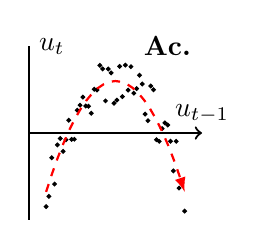
\begin{tikzpicture}[scale=0.11]
		\node at (16, 20) {\textbf{Ac.}}; 
		\draw [thick, ->] (0, 10) -- (20, 10) node [anchor=south] {\( u_{t - 1} \)}; 
		\draw [thick, -] (0, 0) -- (0, 20) node [anchor=west] {\( u_{t} \)}; 
		\draw plot [only marks, mark=*, mark size=6, domain=2:18, samples=50] (\x, {-0.2*(\x - 10)^2 + 13 + 6*rnd}); 
		\draw [thick, dashed, red, -latex] plot [domain=2:18] (\x, {-0.2*(\x - 10)^2 + 16});
	\end{tikzpicture}
\end{center}

\columnbreak

\begin{center}
	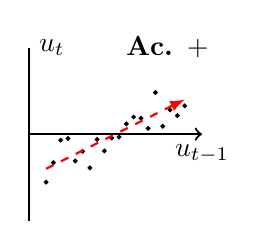
\begin{tikzpicture}[scale=0.11]
		\node at (16, 20) {\textbf{Ac. \( + \)}}; 
		\draw [thick, ->] (0, 10) -- (20, 10) node [anchor=north] {\( u_{t - 1} \)}; 
		\draw [thick, -] (0, 0) -- (0, 20) node [anchor=west] {\( u_{t} \)}; 
		\draw plot [only marks, mark=*, mark size=6, domain=2:18, samples=20] (\x, {5*rnd + 2.5 + 0.5*\x}); 
		\draw [thick, dashed, red, -latex] plot [domain=2:18] (\x, {5 + 0.5*\x});
	\end{tikzpicture}
\end{center}

\columnbreak

\begin{center}
	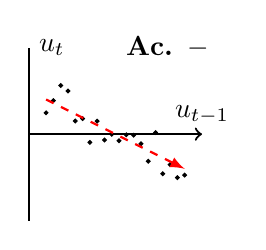
\begin{tikzpicture}[scale=0.11]
		\node at (16, 20) {\textbf{Ac. \( - \)}}; 
		\draw [thick, ->] (0, 10) -- (20, 10) node [anchor=south] {\( u_{t - 1} \)}; 
		\draw [thick, -] (0, 0) -- (0, 20) node [anchor=west] {\( u_{t} \)}; 
		\draw plot [only marks, mark=*, mark size=6, domain=2:18, samples=20] (\x, {5*rnd + 12.5 - 0.5*\x}); 
		\draw [thick, dashed, red, -latex] plot [domain=2:18] (\x, {15 - 0.5*\x});
	\end{tikzpicture}
\end{center}

\end{multicols}

\begin{multicols}{2}

\textbf{Correlogram} - autocorrelation function (ACF) and partial ACF (PACF).

\columnbreak

\begin{itemize}[leftmargin=*]
	\item Y axis: correlation.
	\item X axis: lag number.
	\item Grey area: \( \pm 1.96 / T^{0.5} \)
\end{itemize}

\end{multicols}

\begin{center}
	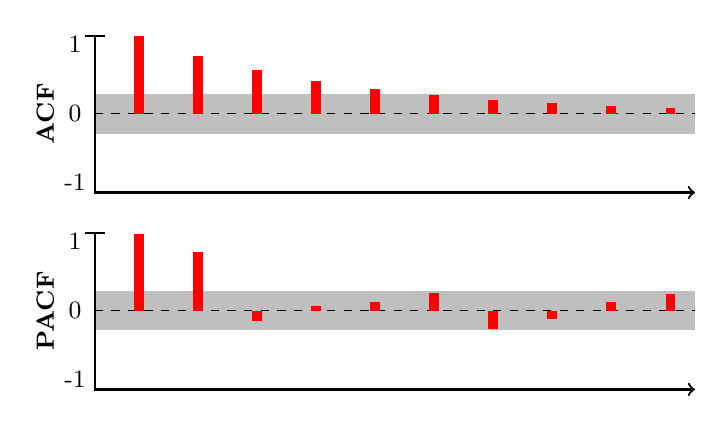
\begin{tikzpicture}[scale=0.25]
		% acf plot
		\node at (-2.5, 14) {\small \rotatebox{90}{\textbf{ACF}}}; 
		\node at (-1, 17.5) {\small 1};
		\node at (-1, 14) {\small 0};
		\node at (-1, 10.5) {\small -1}; 
		\fill [lightgray] (0, 13) rectangle (30.5, 15); 
		\draw [dashed, thin] (0, 14) -- (30.5, 14); 
		\draw [thick, |->] (0, 18) -- (0, 10) -- (30.5, 10);
		\fill [red] (2, 14) rectangle (2.5, 17.95);
		\fill [red] (5, 14) rectangle (5.5, 16.96);
		\fill [red] (8, 14) rectangle (8.5, 16.22); 
		\fill [red] (11, 14) rectangle (11.5, 15.67);
		\fill [red] (14, 14) rectangle (14.5, 15.25);
		\fill [red] (17, 14) rectangle (17.5, 14.94);
		\fill [red] (20, 14) rectangle (20.5, 14.70);
		\fill [red] (23, 14) rectangle (23.5, 14.53);
		\fill [red] (26, 14) rectangle (26.5, 14.40);
		\fill [red] (29, 14) rectangle (29.5, 14.30);
		% pacf plot
		\node at (-2.5, 4) {\small \rotatebox{90}{\textbf{PACF}}};
		\node at (-1, 7.5) {\small 1};
		\node at (-1, 4) {\small 0};
		\node at (-1, 0.5) {\small -1};
		\fill [lightgray] (0, 3) rectangle (30.5, 5);
		\draw [dashed, thin] (0, 4) -- (30.5, 4);
		\draw [thick, |->] (0, 8) -- (0, 0) -- (30.5, 0);
		\fill [red] (2, 4) rectangle (2.5, 7.90);
		\fill [red] (5, 4) rectangle (5.5, 7.00);
		\fill [red] (8, 4) rectangle (8.5, 3.47);
		\fill [red]	(11, 4) rectangle (11.5, 4.24);
		\fill [red] (14, 4) rectangle (14.5, 4.43);
		\fill [red] (17, 4) rectangle (17.5, 4.89);
		\fill [red] (20, 4) rectangle (20.5, 3.09);
		\fill [red] (23, 4) rectangle (23.5, 3.58);
		\fill [red] (26, 4) rectangle (26.5, 4.46);
		\fill [red] (29, 4) rectangle (29.5, 4.86);
	\end{tikzpicture}
\end{center}

\begin{itemize}[leftmargin=*]
	\item \textbf{\( \text{MA}(q) \) process}. \underline{ACF}: only the first \( q \) coefficients are significant, the remaining are abruptly canceled. \underline{PACF}: attenuated exponential fast decay or sine waves.
	\item \textbf{\( \text{AR}(p) \) process}. \underline{ACF}: attenuated exponential fast decay or sine waves. \underline{PACF}: only the first \( p \) coefficients are significant, the remaining are abruptly canceled.
\end{itemize}

\columnbreak

\begin{itemize}[leftmargin=*]
	\item \textbf{\( \text{ARMA}(p, q) \) process}. \underline{ACF} and \underline{PACF}: the coefficients are not abruptly canceled and present a fast decay.
\end{itemize}

If the ACF coefficients do not decay rapidly, there is a clear indicator of a lack of stationarity in mean.

\textbf{Formal tests} - Generally, \( H_{0} \): No autocorrelation.

Supposing that \( u_{t} \) follows an AR(1) process:

\begin{center}
	\( u_{t} = \rho_{1} u_{t - 1} + \varepsilon_{t} \)
\end{center}

where \( \varepsilon_{t} \) is white noise.

\begin{itemize}[leftmargin=*]
	\item \textbf{AR(1) t test} (exogenous regressors):
	\begin{center}
		\( t = \dfrac{\hat{\rho}_{1}}{\se(\hat{\rho}_{1})} \sim t_{T - k - 1, \alpha / 2} \)
	\end{center}
	\( H_{1} \): Autocorrelation of order one, AR(1).
\end{itemize}

\begin{itemize}[leftmargin=*]
	\item \textbf{Durbin-Watson statistic} (exogenous regressors and residual normality):
	\begin{center}
		\( d = \dfrac{\sum_{t = 2}^{n} (\hat{u}_{t} - \hat{u}_{t - 1})^{2}}{\sum_{t = 1}^{n} \hat{u}_{t}^{2}} \approx 2 \cdot (1 - \hat{\rho}_{1}) \)
	\end{center}
	Where \( 0 \leq d \leq 4 \)

	\( H_{1} \): Autocorrelation of order one, AR(1).
\end{itemize}

\begin{center}
	\begin{tabular}{ c | c | c | c }
		\( d = \)          & 0 & 2 & 4  \\ \hline
		\( \rho \approx \) & 1 & 0 & -1
	\end{tabular}

	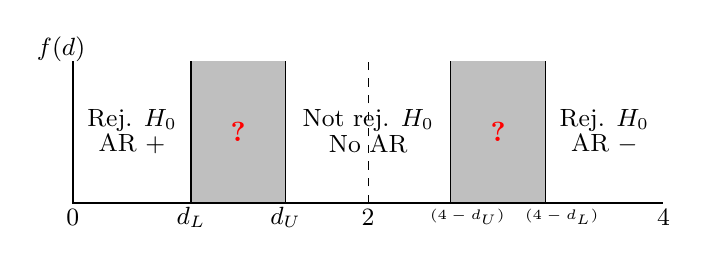
\begin{tikzpicture}[scale=0.3]
		\fill [lightgray] (5, 0) rectangle (9, 6); 
		\draw (5, 0) -- (5, 6);
		\draw (9, 0) -- (9, 6);
		\fill [lightgray] (16, 0) rectangle (20, 6);
		\draw (16, 0) -- (16, 6);
		\draw (20, 0) -- (20, 6);
		\draw [thick] (0, 6) -- (0, 0) -- (25, 0);
		\draw [dashed] (12.5, 0) -- (12.5, 6);
		\node at (-0.5, 6.5) {\small \( f(d) \)};
		\node at (0, -0.6) {\small 0};
		\node at (5, -0.6) {\small \( d_{L} \)};
		\node at (9, -0.6) {\small \( d_{U} \)};
		\node at (12.5, -0.6) {\small 2};
		\node at (16.7, -0.6) {\tiny \( (4 - d_{U}) \)};
		\node at (20.7, -0.6) {\tiny \( (4 - d_{L}) \)};
		\node at (25, -0.6) {\small 4};
		\node at (2.5, 3.5) {\small Rej. \( H_{0} \)};
		\node at (2.5, 2.5) {\small AR \( + \)};
		\node [text=red] at (7, 3) {\textbf{?}};
		\node at (12.5, 3.5) {\small Not rej. \( H_{0} \)};
		\node at (12.5, 2.5) {\small No AR};
		\node [text=red] at (18, 3) {\textbf{?}};
		\node at (22.5, 3.5) {\small Rej. \( H_{0} \)};
		\node at (22.5, 2.5) {\small AR \( - \)};
	\end{tikzpicture}
\end{center}

\begin{itemize}[leftmargin=*]
	\item \textbf{Durbin's h} (endogenous regressors):
	\begin{center}
		\( h = \hat{\rho} \cdot \sqrt{\dfrac{T}{1 - T \cdot \upsilon}} \)
	\end{center}
	where \( \upsilon \) is the estimated variance of the coefficient associated with the endogenous variable.

	\( H_{1} \): Autocorrelation of order one, AR(1).
\end{itemize}

\begin{itemize}[leftmargin=*]
	\item \textbf{Breusch-Godfrey test} (endogenous regressors): it can detect \( \text{MA}(q) \) and \( \text{AR}(p) \) processes (\( \varepsilon_{t} \) is w. noise):
	\begin{itemize}[leftmargin=*]
		\item \( \text{MA}(q) \): \( u_{t} = \varepsilon_{t} - m_{1} u_{t - 1} - \cdots - m_{q} u_{t - q} \)
		\item \( \text{AR}(p) \): \( u_{t} = \rho_{1} u_{t - 1} + \cdots + \rho_{p} u_{t - p}+ \varepsilon_{t} \)
	\end{itemize}
	Under \( H_{0} \): No autocorrelation:
	\begin{center}
		\( \hfill T \cdot R_{\hat{u}_t}^{2} \underset{a}{\sim} \chi_{q}^{2} \hfill \text{or} \hfill T \cdot R_{\hat{u}_t}^{2} \underset{a}{\sim} \chi_{p}^{2} \hfill \)
	\end{center}
	\( H_{1} \): Autocorrelation of order \( q \) (or \( p \)).
\end{itemize}

\begin{itemize}[leftmargin=*]
	\item \textbf{Ljung-Box Q test}:

	\( H_{1} \): Autocorrelation up to lag \( h \).
\end{itemize}

\columnbreak

\subsection*{Correction}

\begin{itemize}[leftmargin=*]
	\item Use OLS with a variance-covariance matrix estimator that is \textbf{robust to heteroscedasticity and autocorrelation} (HAC), for example, the one proposed by \textbf{Newey-West}.
	\item Use \textbf{Generalized Least Squares} (GLS). Supposing \( y_{t} = \beta_{0} + \beta_{1} x_{t} + u_{t} \), with \( u_{t} = \rho u_{t - 1} + \varepsilon_{t} \), where \( \lvert \rho \rvert < 1 \) and \( \varepsilon_{t} \) is \underline{white noise}.
	\begin{itemize}[leftmargin=*]
		\item If \( \rho \) is \textbf{known}, use a \textbf{quasi-differentiated model}:
		\begin{center}
			\( y_{t} - \rho y_{t - 1}= \beta_{0} (1 - \rho) + \beta_{1} (x_{t} - \rho x_{t - 1}) + u_{t} - \rho u_{t - 1} \)

			\( y_{t}^{*} = \beta_{0}^{*} + \beta_{1}' x_{t}^{*} + \varepsilon_{t} \)
		\end{center}
		where \( \beta_{1}' = \beta_{1} \); and estimate it by OLS.
		\item If \( \rho \) is \textbf{not known}, estimate it by -for example- the \textbf{Cochrane-Orcutt iterative method} (Prais-Winsten's method is also good):
		\begin{enumerate}[leftmargin=*]
			\item Obtain \( \hat{u}_{t} \) from the original model.
			\item Estimate \( \hat{u}_{t} = \rho \hat{u}_{t - 1} + \varepsilon_{t} \) and obtain \( \hat{\rho} \).
			\item Create a quasi-differentiated model:
			\begin{center}
				\( y_{t} - \hat{\rho}y_{t - 1} = \beta_{0} (1 - \hat{\rho}) + \beta_{1} (x_{t} - \hat{\rho} x_{t - 1}) + u_{t} - \hat{\rho}u_{t - 1} \)

				\( y_{t}^{*} = \beta_{0}^{*} + \beta_{1}' x_{t}^{*} + \varepsilon_{t} \)
			\end{center}
			where \( \beta_{1}' = \beta_{1} \); and estimate it by OLS.
			\item Obtain \( \hat{u}_{t}^{*} = y_{t} - (\hat{\beta}_{0}^{*} + \hat{\beta}_{1}' x_{t}) \neq y_{t} - (\hat{\beta}_{0}^{*} + \hat{\beta}_{1}' x_{t}^{*}) \).
			\item Repeat from step 2. The algorithm ends when the estimated parameters vary very little between iterations.
		\end{enumerate}
	\end{itemize}
	\item If not solved, look for \textbf{high dependence} in the series.
\end{itemize}

\section*{Exponential smoothing}

Given \( \{ y_{t} \} \), the smoothed series \( \{ f_{t} \} \):

\begin{center}
	\( f_{t} = \alpha y_{t} + (1 - \alpha) f_{t - 1} \)
\end{center}

where \( 0 < \alpha < 1 \) is the smoothing factor and \( f_{0} = y_{0} \).

\section*{Predictions}

Two types of predictions:

\begin{itemize}[leftmargin=*]
	\item Of the mean value of \( y \) for a specific value of \( x \).
	\item Of an individual value of \( y \) for a specific value of \( x \).
\end{itemize}

\textbf{Theil's U statistic} - compares the forecast results with the ones of forecasting with minimal historical data.

\begin{center}
	\( U = \sqrt{\frac{\sum_{t = 1}^{T - 1} \left( \frac{\hat{y}_{t + 1} - y_{t + 1}}{y_{t}} \right)^{2}}{\sum_{t = 1}^{T - 1} \left( \frac{y_{t + 1} - y_{t}}{y_{t}} \right)^{2}}} \)
\end{center}

\begin{itemize}[leftmargin=*]
	\item \( < 1 \): The forecast is better than guessing.
	\item \( = 1 \): The forecast is about as good as guessing.
	\item \( > 1 \): The forecast is worse than guessing.
\end{itemize}

\columnbreak

\section*{Stationarity}

Stationarity allows to correctly identify relations --that stay unchanged with time-- between variables.

\begin{itemize}[leftmargin=*]
	\item \textbf{Stationary process} (strict stationarity) - the joint probability distribution of the process remains unchanged when shifted \( h \) periods.
	\item \textbf{Non-stationary process} - for example, a series with trend, where at least the mean changes with time.
	\item \textbf{Covariance stationary process} - it is a weaker form of stationarity:
	\begin{itemize}[leftmargin=*]
		\begin{multicols}{2}
			\item \( \E(x_{t}) \) is constant.
		\columnbreak
			\item \( \Var(x_{t}) \) is constant.
		\end{multicols}
		\item For any \( t, h \geq 1 \), \( \Cov(x_{t}, x_{t + h}) \) depends only of \( h \), not of \( t \).
	\end{itemize}
\end{itemize}

\section*{Weak dependence}

Weak dependence replaces the random sampling assumption for time series.

\begin{itemize}[leftmargin=*]
	\item An stationary process \( \{ x_{t} \} \) is \textbf{weakly dependent} when \( x_{t} \) and \( x_{t + h} \) are almost independent as \( h \) increases without a limit.
	\item A covariance stationary process is \textbf{weakly dependent} if the correlation between \( x_{t} \) and \( x_{t + h} \) tends to 0 fast enough when \( h \rightarrow \infty \) (they are not asymptotically correlated).
\end{itemize}

Weakly dependent processes are known as \textbf{integrated of order zero}, I(0). Some examples:

\begin{itemize}[leftmargin=*]
	\item \textbf{Moving average} - \( \{ x_{t} \} \) is a moving average of order \( q \), \( \text{MA}(q) \):
	\begin{center}
		\( x_{t} = e_{t} + m_{1} e_{t - 1} + \cdots + m_{q} e_{t - q} \)
	\end{center}
	where \( \{ e_{t} : t = 0, 1, \ldots, T \} \) is an \textsl{i.i.d.} sequence with zero mean and \( \sigma_{e}^{2} \) variance.
	\item \textbf{Autoregressive process} - \( \{ x_{t} \} \) is an autoregressive process of order \( p \), \( \text{AR}(p) \):
	\begin{center}
		\( x_{t} = \rho_{1} x_{t - 1} + \cdots + \rho_{p} x_{t - p} + e_{t} \)
	\end{center}
	where \( \{ e_{t} : t = 1, 2, \ldots, T \} \) is an \textsl{i.i.d.} sequence with zero mean and \( \sigma_{e}^{2} \) variance.

	\textbf{Stability condition}: if \( 1 - \rho_{1} z - \cdots - \rho_{p} z^{p} = 0 \) for \( \lvert z \rvert > 1 \) then \( \{ x_{t} \} \) is an \( \text{AR}(p) \) stable process that is weakly dependent. For AR(1), the condition is: \( \lvert \rho_{1} \rvert < 1 \).

	\item \textbf{ARMA process} - is a combination of the previous; \( \{ x_{t} \} \) is an \( \text{ARMA}(p, q) \):
	\begin{center}
		\( x_{t} = e_{t} + m_{1} e_{t - 1} + \cdots + m_{q} e_{t - q} + \rho_{1} x_{t - 1} + \cdots + \rho_{p} x_{t - p} \)
	\end{center}
\end{itemize}

\columnbreak

\section*{Unit roots}

A process is integrated of order \( d \), \( \text{I}(d) \), if applying differences \( d \) times makes the process stationary.

When \( d \geq 1 \), the process is said to have a \textbf{unit root}. A process has a unit root when the stability condition is not met (there are roots on the unit circle).

\subsection*{Strong dependence}

Generally, economic series are highly persistent in time. Some examples of \textbf{unit root} I(1):

\begin{itemize}[leftmargin=*]
	\item \textbf{Random walk} - an AR(1) process with \( \rho_{1} = 1 \).
	\begin{center}
		\( y_{t} = y_{t - 1} + e_{t} \)
	\end{center}
	where \( \{ e_{t} : t = 1, 2, \ldots, T \} \) is an \textsl{i.i.d.} sequence with zero mean and \( \sigma_{e}^{2} \) variance.
	\item \textbf{Random walk with a drift} - an AR(1) process with \( \rho_{1} = 1 \) and a constant.
	\begin{center}
		\( y_{t} = \beta_{0} + y_{t - 1} + e_{t} \)
	\end{center}
	where \( \{ e_{t} : t = 1, 2, \ldots, T \} \) is an \textsl{i.i.d.} sequence with zero mean and \( \sigma_{e}^{2} \) variance.
\end{itemize}

\subsection*{Unit root tests}

\begin{center}
	\begin{tabular}{ c | c | c }
		Test            & \( H_{0} \) & Reject \( H_{0} \)                 \\ \hline
		ADF             & I(1)        & tau \textless \, Critical value    \\ \hline
		KPSS            & I(0) level  & mu \textgreater \, Critical value  \\
		                & I(0) trend  & tau \textgreater \, Critical value \\ \hline
		Phillips-Perron & I(1)        & Z-tau \textless \, Critical value  \\ \hline
		Zivot-Andrews   & I(1)        & tau \textless \, Critical value
	\end{tabular}
\end{center}

\subsection*{From unit root to weak dependence}

Integrated of \textbf{order one}, I(1), means that \textbf{the first difference} of the process is \textbf{weakly dependent} or I(0) (and usually, stationary). Let \( \{ y_{t} \} \) be a random walk:

\begin{multicols}{2}

\begin{center}
	\( \Delta y_{t} = y_{t} - y_{t - 1} = e_{t} \)
\end{center}

where \( \{ e_{t} \} = \{ \Delta y_{t} \} \) is \textsl{i.i.d.}

Note:

\begin{itemize}[leftmargin=*]
	\item The {\color{red} first difference} of a series removes its trend.
	\item Logarithms of a series stabilizes its variance.
\end{itemize}

\columnbreak

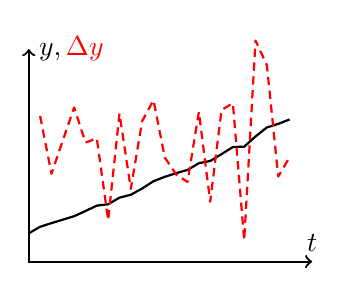
\begin{tikzpicture}[scale=0.18]
	\draw [thick, <->] (0, 15) node [anchor=west] {\( y, {\color{red} \Delta y} \)} -- (0, 0) -- (20, 0) node [anchor=south] {\( t \)}; 
	\draw [thick, black] 
	(0.0, 2.000) -- (0.8, 2.459) -- 
	(1.6, 2.716) -- (3.2, 3.205) -- 
	(4.0, 3.571) -- (4.8, 3.952) -- 
	(5.6, 4.047) -- (6.4, 4.514) -- 
	(7.2, 4.719) -- (8.0, 5.160) -- 
	(8.8, 5.674) -- (9.6, 5.987) -- 
	(10.4, 6.242) -- (11.2, 6.471) -- 
	(12.0, 6.944) -- (12.8, 7.104) -- 
	(13.6, 7.584) -- (14.4, 8.087) -- 
	(15.2, 8.112) -- (16.0, 8.834) -- 
	(16.8, 9.470) -- (17.6, 9.718) -- 
	(18.4, 10.032); 
	\draw [thick, red, densely dashed, line join=round]
	(0.8, 10.28) -- (1.6, 6.20) -- 
	(3.2, 10.88) -- (4.0, 8.40) -- 
	(4.8, 8.70) -- (5.6, 2.92) -- 
	(6.4, 10.45) -- (7.2, 5.13) -- 
	(8.0, 9.92) -- (8.8, 11.39) -- 
	(9.6, 7.34) -- (10.4, 6.15) -- 
	(11.2, 5.62) -- (12.0, 10.57) -- 
	(12.8, 4.23) -- (13.6, 10.70) -- 
	(14.4, 11.18) -- (15.2, 1.51) -- 
	(16.0, 15.60) -- (16.8, 13.86) -- 
	(17.6, 6.01) -- (18.4, 7.36);
\end{tikzpicture}

\end{multicols}

\subsubsection*{From unit root to percentage change}

When an I(1) series is strictly positive, logs are often used before differencing to approximate percentage changes:

\begin{center}
	\( \Delta \log(y_{t}) = \log(y_{t}) - \log(y_{t - 1}) \approx \dfrac{y_t - y_{t - 1}} {y_{t - 1}} \)
\end{center}

\columnbreak

\subsection*{Ergodicity}

A strictly stationary process \( \{ y_{t} \} \) is \textbf{ergodic} if time averages converge to their ensemble averages (expectations). This is often ensured by \textbf{strong mixing}, which implies asymptotic independence of distant events.

\begin{center}
	\( \frac{1}{T} \sum_{t = 1}^{T} y_{t} \underset{a}{\rightarrow} \E(y_{t}) \)
\end{center}

Without it, sample moments may not reflect population moments. Estimators are inconsistent.

\section*{Cointegration}

Two I(1) series are \textbf{cointegrated} if a linear combination is I(0). In that case, a regression between them is not spurious but reflects a valid \textbf{long-run} relationship. Cointegrated variables share a common stochastic trend.

For example, \( \{ x_{t} \} \) and \( \{ y_{t} \} \) are I(1), but \( y_{t} - \beta x_{t} = u_{t} \) where \( \{ u_{t} \} \) is I(0). (\( \beta \) is the cointegrating parameter).

\subsection*{Cointegration test}

\begin{enumerate}[leftmargin=*]
	\item Estimate \( y_{t} = \alpha + \beta x_{t} + \varepsilon_{t} \) and obtain \( \hat{\varepsilon}_{t} \).
	\item Perform an ADF test on \( \hat{\varepsilon}_{t} \) with a modified distribution.
	The result of this test is equivalent to:
	\begin{itemize}[leftmargin=*]
		\item \( H_{0} \): \( \beta = 0 \) (no cointegration)
		\item \( H_{1} \): \( \beta \neq 0 \) (cointegration)
	\end{itemize}
	if test statistic \( > \) critical value, reject \( H_{0} \).
\end{enumerate}

\section*{Heteroscedasticity in time series}

The \textbf{assumption} affected is \textbf{t4}, which leads \textbf{OLS to be not efficient}.

Use tests like Breusch-Pagan or White's, where \( H_{0} \): No heteroscedasticity. For these tests to work, there should be \textbf{no autocorrelation}.

\subsection*{ARCH}

An autoregressive conditional heteroscedasticity (ARCH) model is used to analyze a form of dynamic heteroscedasticity, where the error variance follows an \( \text{AR}(p) \) process.

Given the model: \( y_{t} = \beta_{0} + \beta_{1} z_{t} + u_{t} \) where, there is AR(1) and heteroscedasticity:

\begin{center}
	\( \E(u_{t}^{2} \mid u_{t - 1}) = \alpha_{0} + \alpha_{1} u_{t - 1}^{2} \)
\end{center}

\subsection*{GARCH}

A general ARCH (GARCH) model is similar to ARCH, but the error variance follows an \( \text{ARMA}(p, q) \) process.

\end{multicols}

\end{document}